\documentclass[../main.tex]{subfiles}


\begin{document}
\raggedright

\subsection{Basic Web}

	\begin{figure}[!htb]
        \center{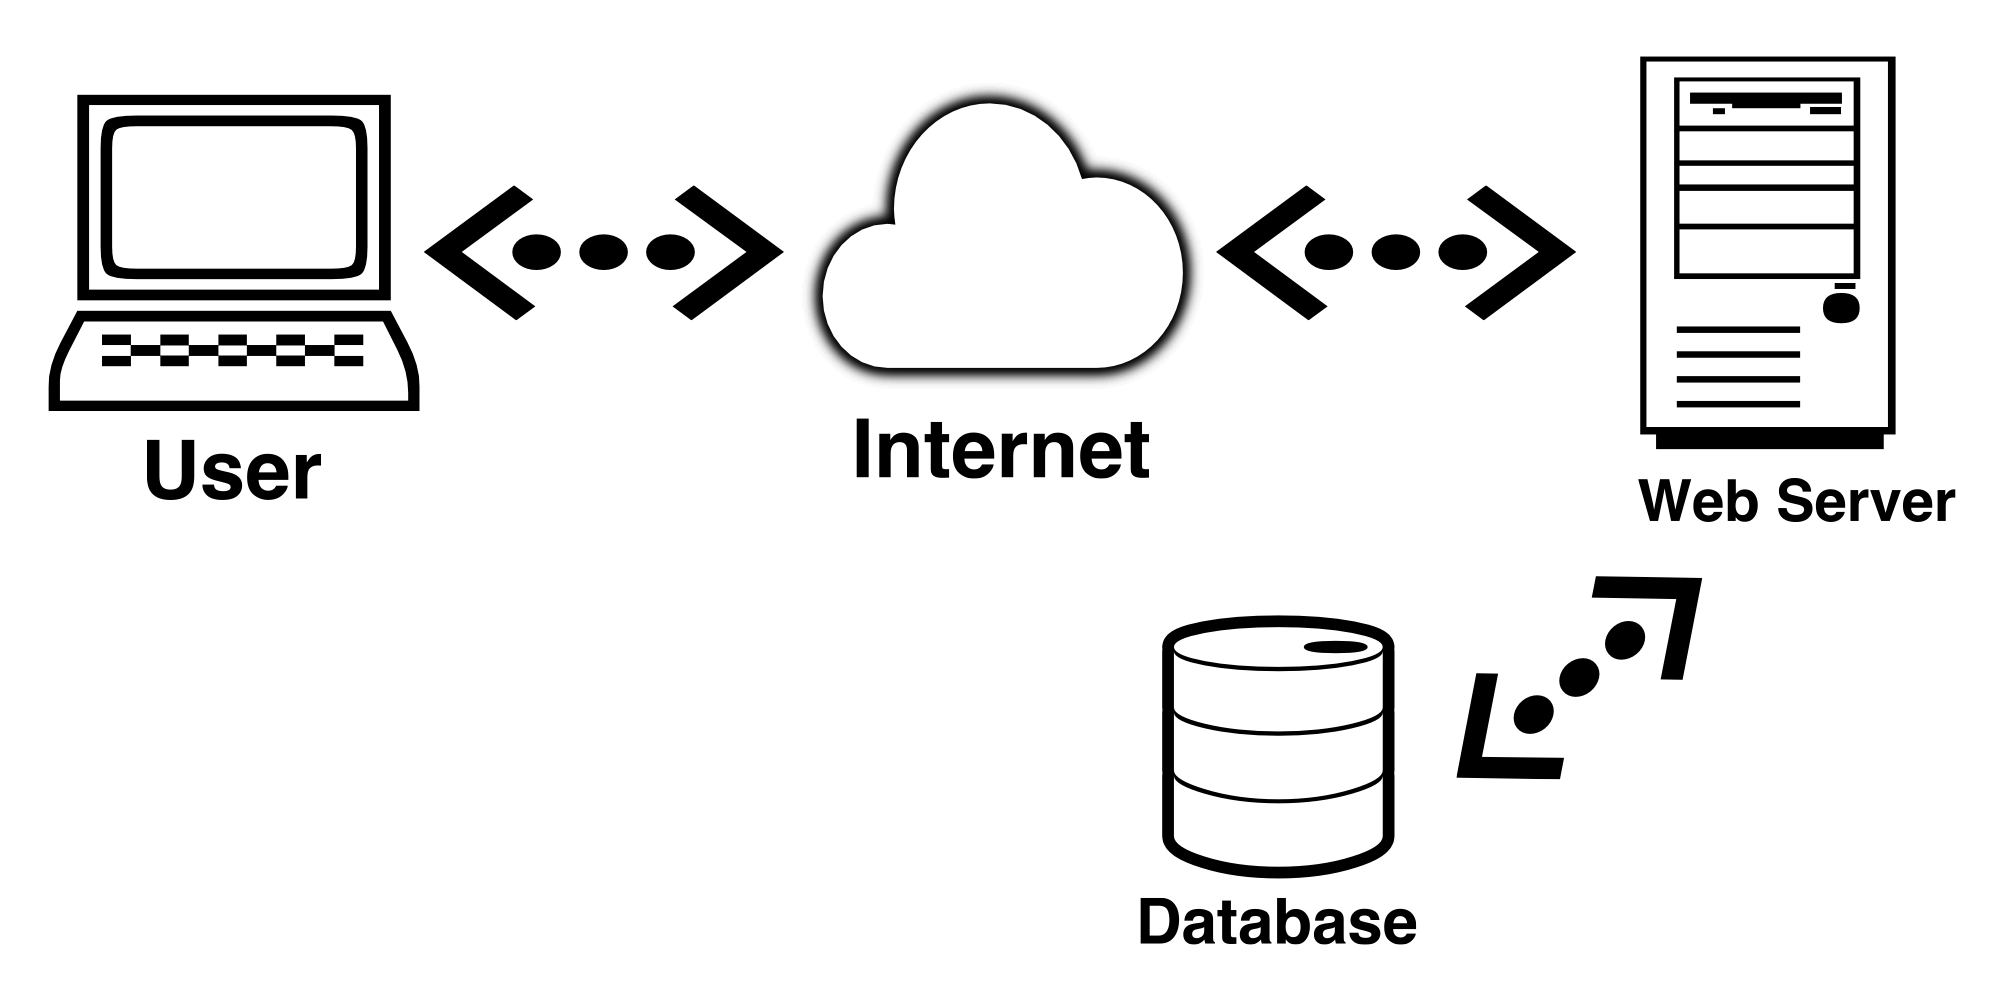
\includegraphics[scale=0.25]
        {images/webserverdesign.png}}
        \caption{\label{fig:basicwebdesign} Basic Web Server.}
      \end{figure}
      
Figure~\ref{fig:basicwebdesign} shows the basic version of how a web server works. The user makes a request via their Internet Service Provider(ISP) onto the internet and that then connects to the web server hosting the site built and the database connected to it. Once the relevant information has been retrieved the server forwards it back to the internet and it is received by the user. Having a system like this would allow the user to access all data from any device, screen size, and hardware that is able to connect to the internet making it very flexible and easy to use.
      
\subsection{The System}
      
Web-Based systems are spread into various different languages with both positives and negatives. Java, .NET, PHP, ASP, Python, Ruby, ColdFusion are just a few of the most used language examples for web systems\cite{securelanguage}. Figure~\ref{fig:mostlanguagesused} and Figure~\ref{fig:languageattacks} shows us programming languages that are widely used for web systems and a comparison of their vulnerabilities. Selecting a secure language is an important aspect for security and confidentiality of this project.  \\[2mm]


\begin{figure}[H]
        \center{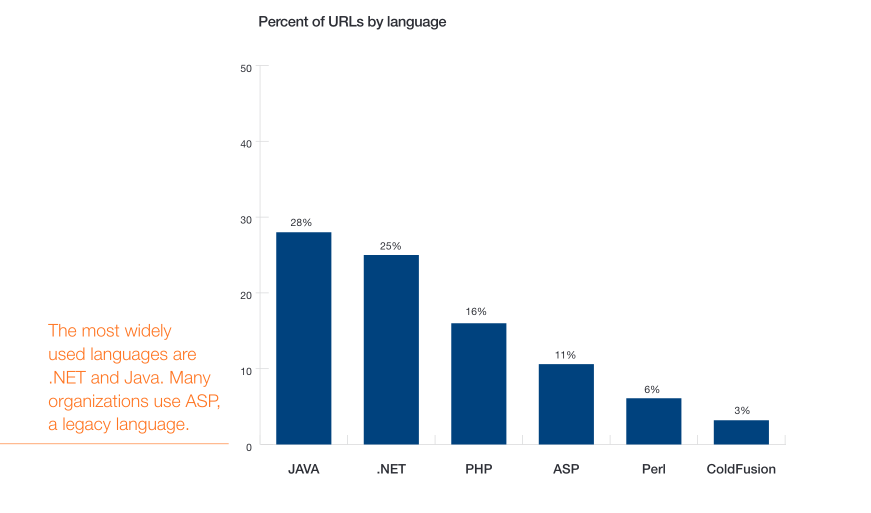
\includegraphics[scale=0.6]
        {images/mostLanguagesUsed.png}}
        \caption{\label{fig:mostlanguagesused} Most widely used languages for Web Systems - WhiteHatSec\cite{WhiteHatSec}}
      \end{figure}


With all these languages, the highest priority would be to find a language which has Cyber Security as one of its strong points. .NET, Java, ASP, PHP all come with a high number of vulnerabilities as they are highly used\cite{securelanguage}.  \\[2mm]

\begin{figure}[!h]
        \center{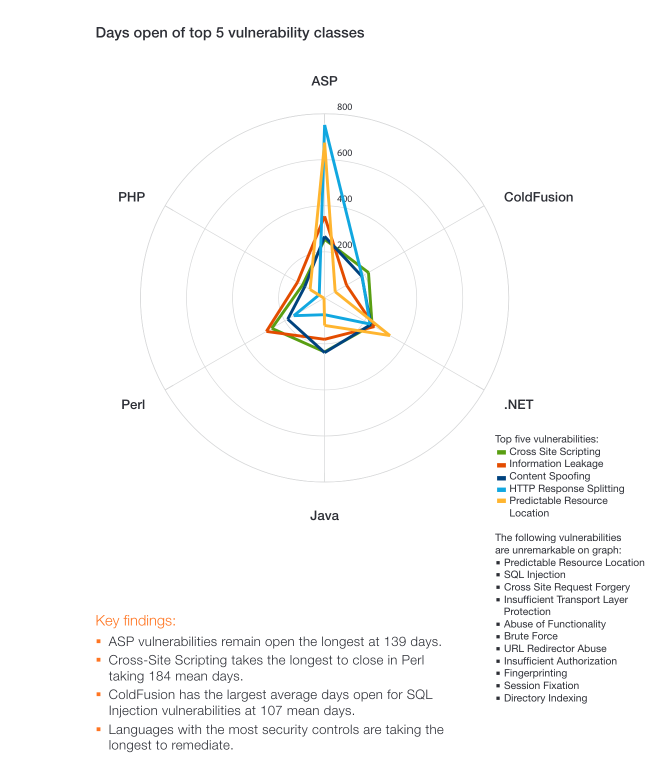
\includegraphics[scale=0.75]
        {images/languageAttacks.png}}
        \caption{\label{fig:languageattacks} Security Vulnerabilites in ASP, PHP, Perl, Java, .NET and ColdFusion - WhiteHatSec\cite{WhiteHatSec}}
      \end{figure}

This would then leave us with Python and Ruby which are both easy to code with and used widely. Using a web framework of the languages, Django(Python) or Ruby On Rails(Ruby) would be a smart idea because frameworks allow increased security as they are built for this and increase the efficiency and are cost effective\cite{djangovslaravel}. 




\end{document}
